\documentclass{ximera}

%\addPrintStyle{..}

\begin{document}
	\author{Bart Lambregs}
	\xmtitle{Eenparige versnelde rechtlijnige beweging}{}
    \xmsource\xmuitleg



De ééndimensionale beweging met een constante  versnelling wordt de \textit{eenparig veranderlijke rechtlijnige beweging}, afgekort EVRB, genoemd. 
Eenparig betekent gelijkmatig; bij een constante versnelling is de \textit{verandering} van de snelheid steeds gelijk.
De grafiek van $a(t)=a$ is een constante met $a$ een reëel getal is.
Ook voor deze beweging kan je de plaatsfunctie en snelheidsfunctie bepalen en zo het verloop van de plaats en snelheid in functie van de tijd kennen. 


% Een eendimensionale beweging met constante versnelling noemt de  \textit{eenparig veranderlijke rechtlijnige beweging} (EVRB). 
% Eenparig betekent gelijkmatig; de snelheidsverandering is steeds gelijk. De grafiek van $a(t)=a$ is een constante functie waarbij $a$ een reëel getal is. 
% Ook voor deze beweging kan je de plaatsfunctie en snelheidsfunctie bepalen en zo het verloop van de plaats en snelheid in functie van de tijd kennen. 


Voor \(t_0 = 0\) worden de gemiddelde snelheid en versnelling gegeven door: 

\[
\bar{v} = \frac{\Delta x}{\Delta t} = \frac{x - x_0}{t - t_0} = \frac{x - x_0}{t}
\]

\[
a = \frac{\Delta v}{\Delta t} = \frac{v - v_0}{t - t_0} = \frac{v - v_0}{t}
\]


\begin{quickquestion*}{}{}
Waarom geldt er dat voor de EVRB dat \( \overline{a} = a\)? 
\end{quickquestion*}

Deze formules omvormen levert een eerstegraadsvergelijking in de veranderlijke \(t\): 

\[
x = x_0 + \bar{v}t 
\]

\[
v = v_0 + at 
\]

% HIER KAN EEN TIKZ PICTURE DUIDELIJKHEID BRENGEN; IS EIGENLIJK NIET MEER DAN DE SYMETRIE VAN EEN RECHT LIJNSTUK 
% MISSCHIEN IS DIT TE MOEILIJK.. 

De snelheid \(v = v_0 + at \) is een lineaire functie, in oefening X van vorig hoofdstuk werd aangetoond dat de gemiddelde snelheid geschreven dan kan worden als: 

\[
\bar{v} = \frac{v_0 + v}{2} 
\]



Dit alles invullen in de plaatsfunctie levert: 

\begin{align*}
	x &= x_0 + \bar{v}t \\
	  &= x_0 + \left( \frac{v_0 + v}{2} \right)t \\
	  &= x_0 + \left( \frac{v_0 + v_0 + at}{2} \right)t \\
	  &= x_0 + v_0 t + \frac{1}{2} at^2
\end{align*}

\[
\Rightarrow \quad x = x_0 + v_0 t + \frac{1}{2}at^2 
\]

\begin{quickquestion*}{}{}
	Verklaar in elke tussenstap welke formule er wordt ingevuld. 
\end{quickquestion*}


\begin{theorem}
De plaatsfunctie $x(t)$ en de snelheidsfunctie $v(t)$ van een EVRB met versnelling $a$ worden gegeven door:
\[
\begin{array}{rcl}
x(t)&=&x_0+v_0t+\frac{1}{2}at^2\\
v(t)&=&v_0+at
\end{array}
\]
Hierin is $x_0$ de \textit{beginpositie} en $v_0$ de \textit{beginsnelheid}. Ze worden bepaald door de \textit{beginvoorwaarden} of \textit{randvoorwaarden}.
\end{theorem}	

Indien de beschrijving van de beweging niet op $t=0$ start maar op een gegeven tijdstip $t_0$, dan wordt in de beschrijving $t$ vervangen door $\Delta t= t-t_0$, de verstreken tijd vanaf het begintijdstip $t_0$. De plaatsfunctie en zijn afgeleide worden dan een klein beetje ingewikkelder:

\[
\begin{array}{rcl}
x(t)&=&x_0+v_0(t-t_0)+\frac{1}{2}a(t-t_0)^2\\
v(t)&=&v_0+a(t-t_0)
\end{array}
\]



\begin{exercise}
	Hoe werden de 
\end{exercise}





Met de functies kan je de volgende formule voor de gemiddelde snelheid van een EVRB aantonen:%\footnote{Het formuletje is handig te gebruiken in veel vraagstukken door gebruik te maken van $\Delta x=\overline{v}\Delta t$.} 
\footnote{De afleiding van de gemiddelde snelheid is als volgt:
\begin{eqnarray*}
\overline{v}=\frac{\Delta x}{\Delta t}=\frac{x-x_0}{t-t_0}=\frac{v_0(t-t_0)+\frac{1}{2}a(t-t_0)^2}{(t-t_0)}=\frac{2v_0+a(t-t_0)}{2}=\frac{v_0+v}{2}.
\end{eqnarray*}}

\[
\overline{v}=\frac{v_0+v}{2}
\]

Blijkbaar houdt het eenparig toenemen van de snelheid in dat we het rekenkundig gemiddelde kunnen gebruiken voor de gemiddelde snelheid.



\begin{quickquestion*}{}{}
\begin{itemize}
	\item Op het moment\(t_1\) de snelheid gelijk aan nul, is de versnelling dan ook gelijk aan nul? 
	\item Op het moment\(t_1\) de vernelling gelijk aan nul, is de snelheid dan ook gelijk aan nul? 
	\item Als een auto vertraagd, is de versnelling dan negatief? 
\end{itemize}
\end{quickquestion*}

\begin{image}

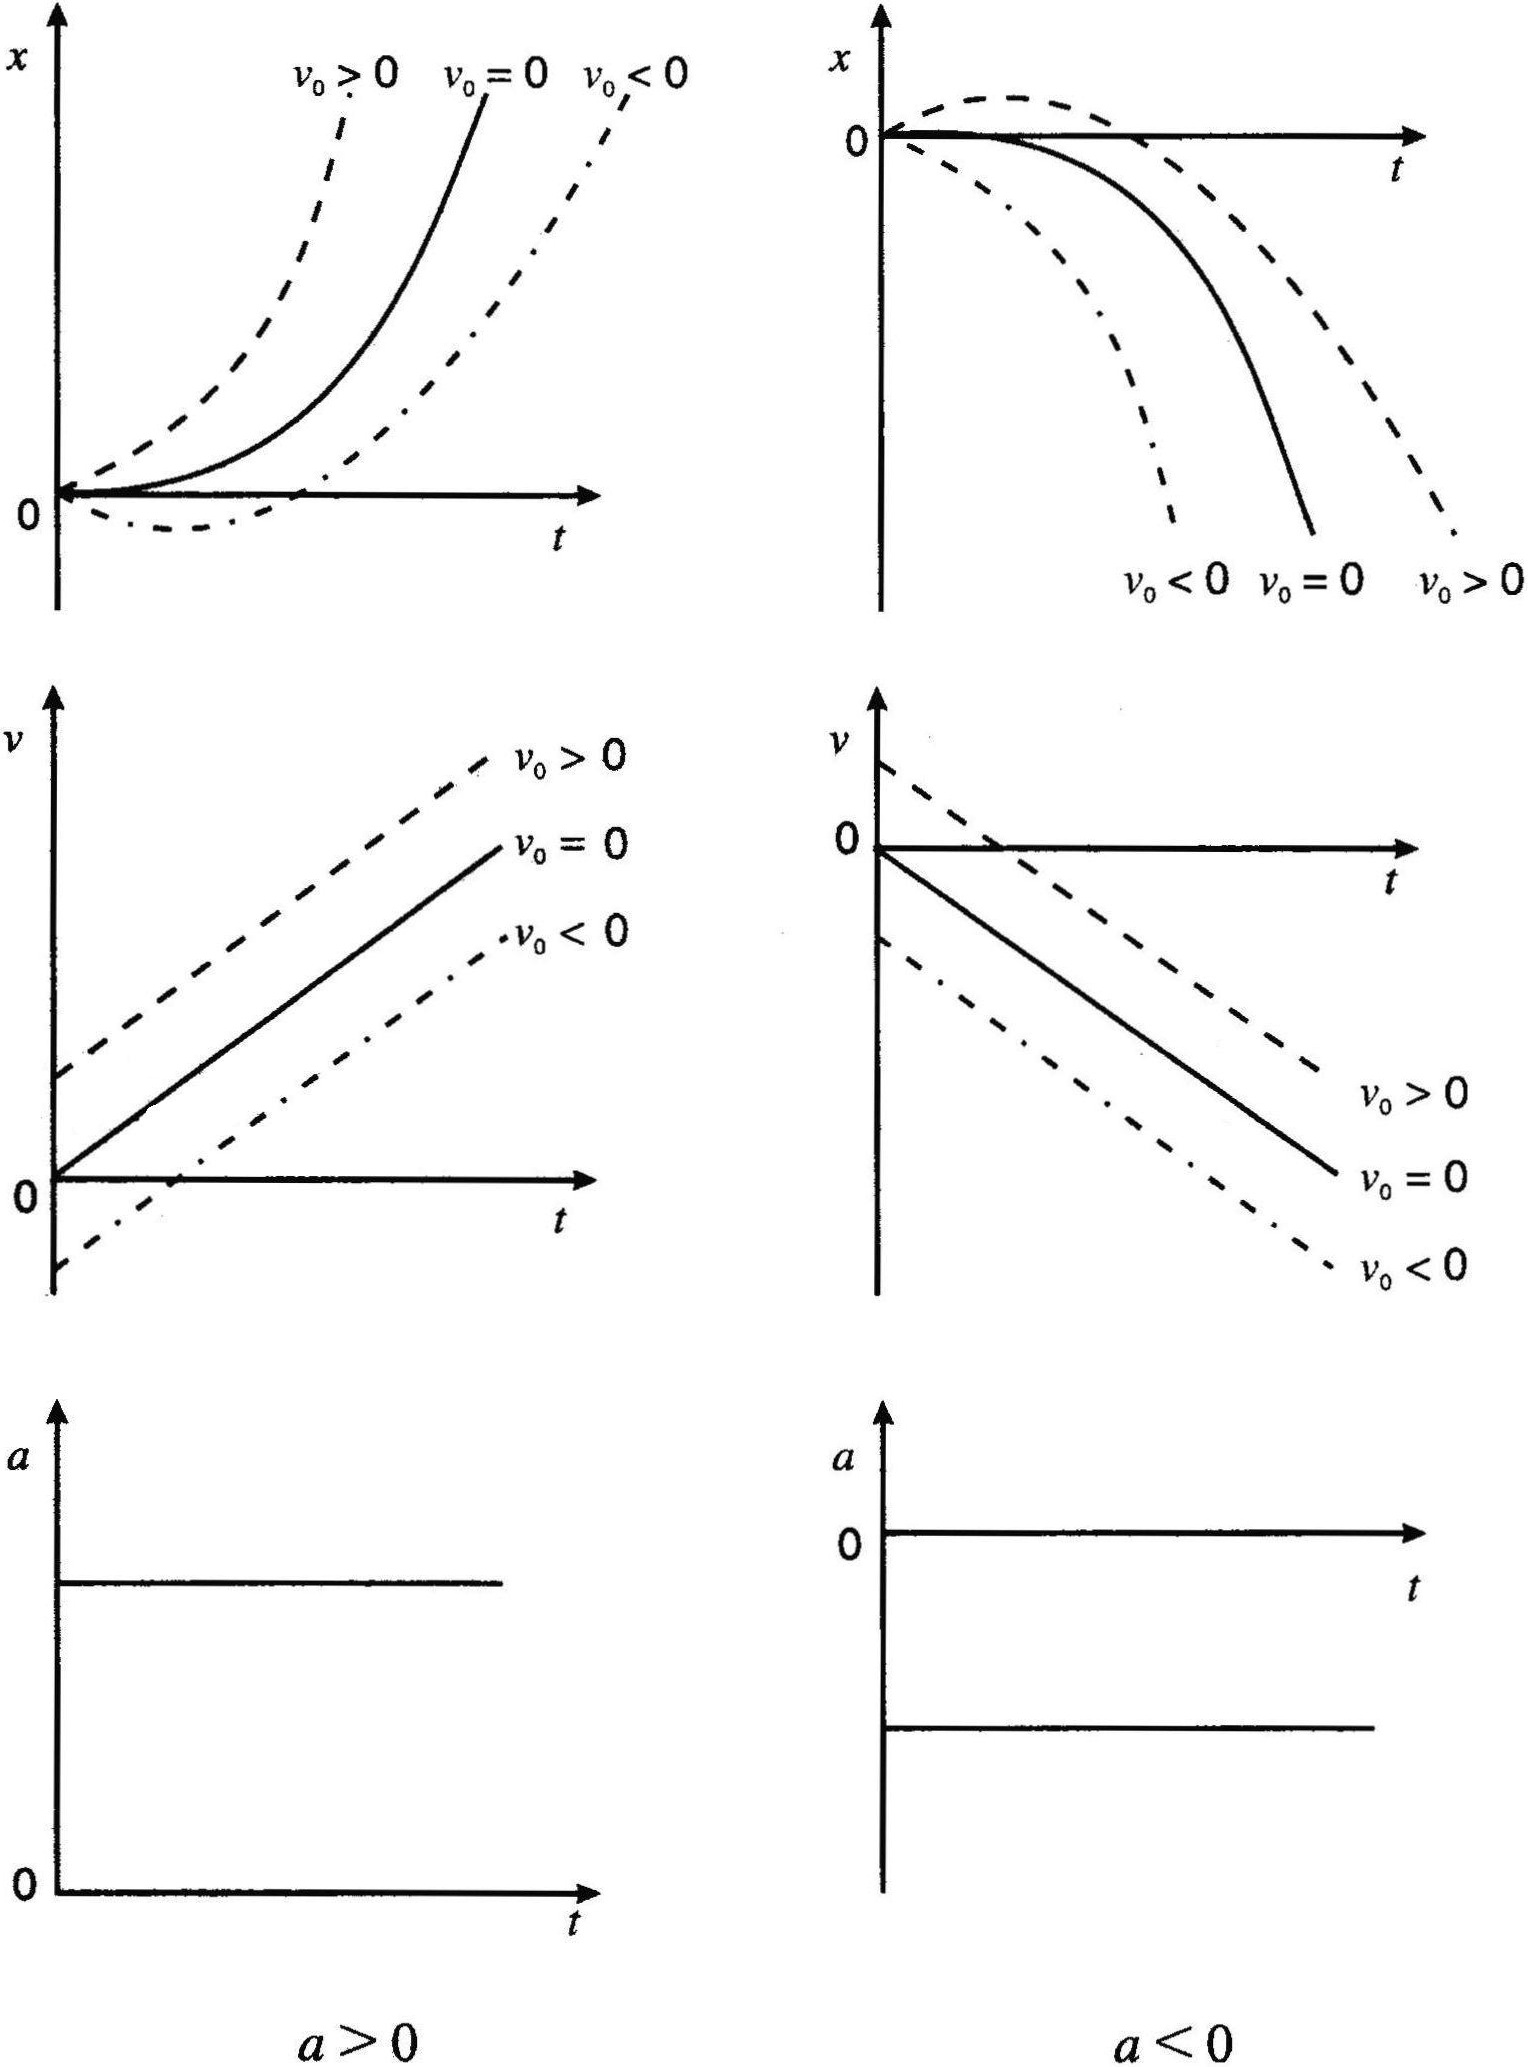
\includegraphics[width=\textwidth]{EVRB_grafieken}
%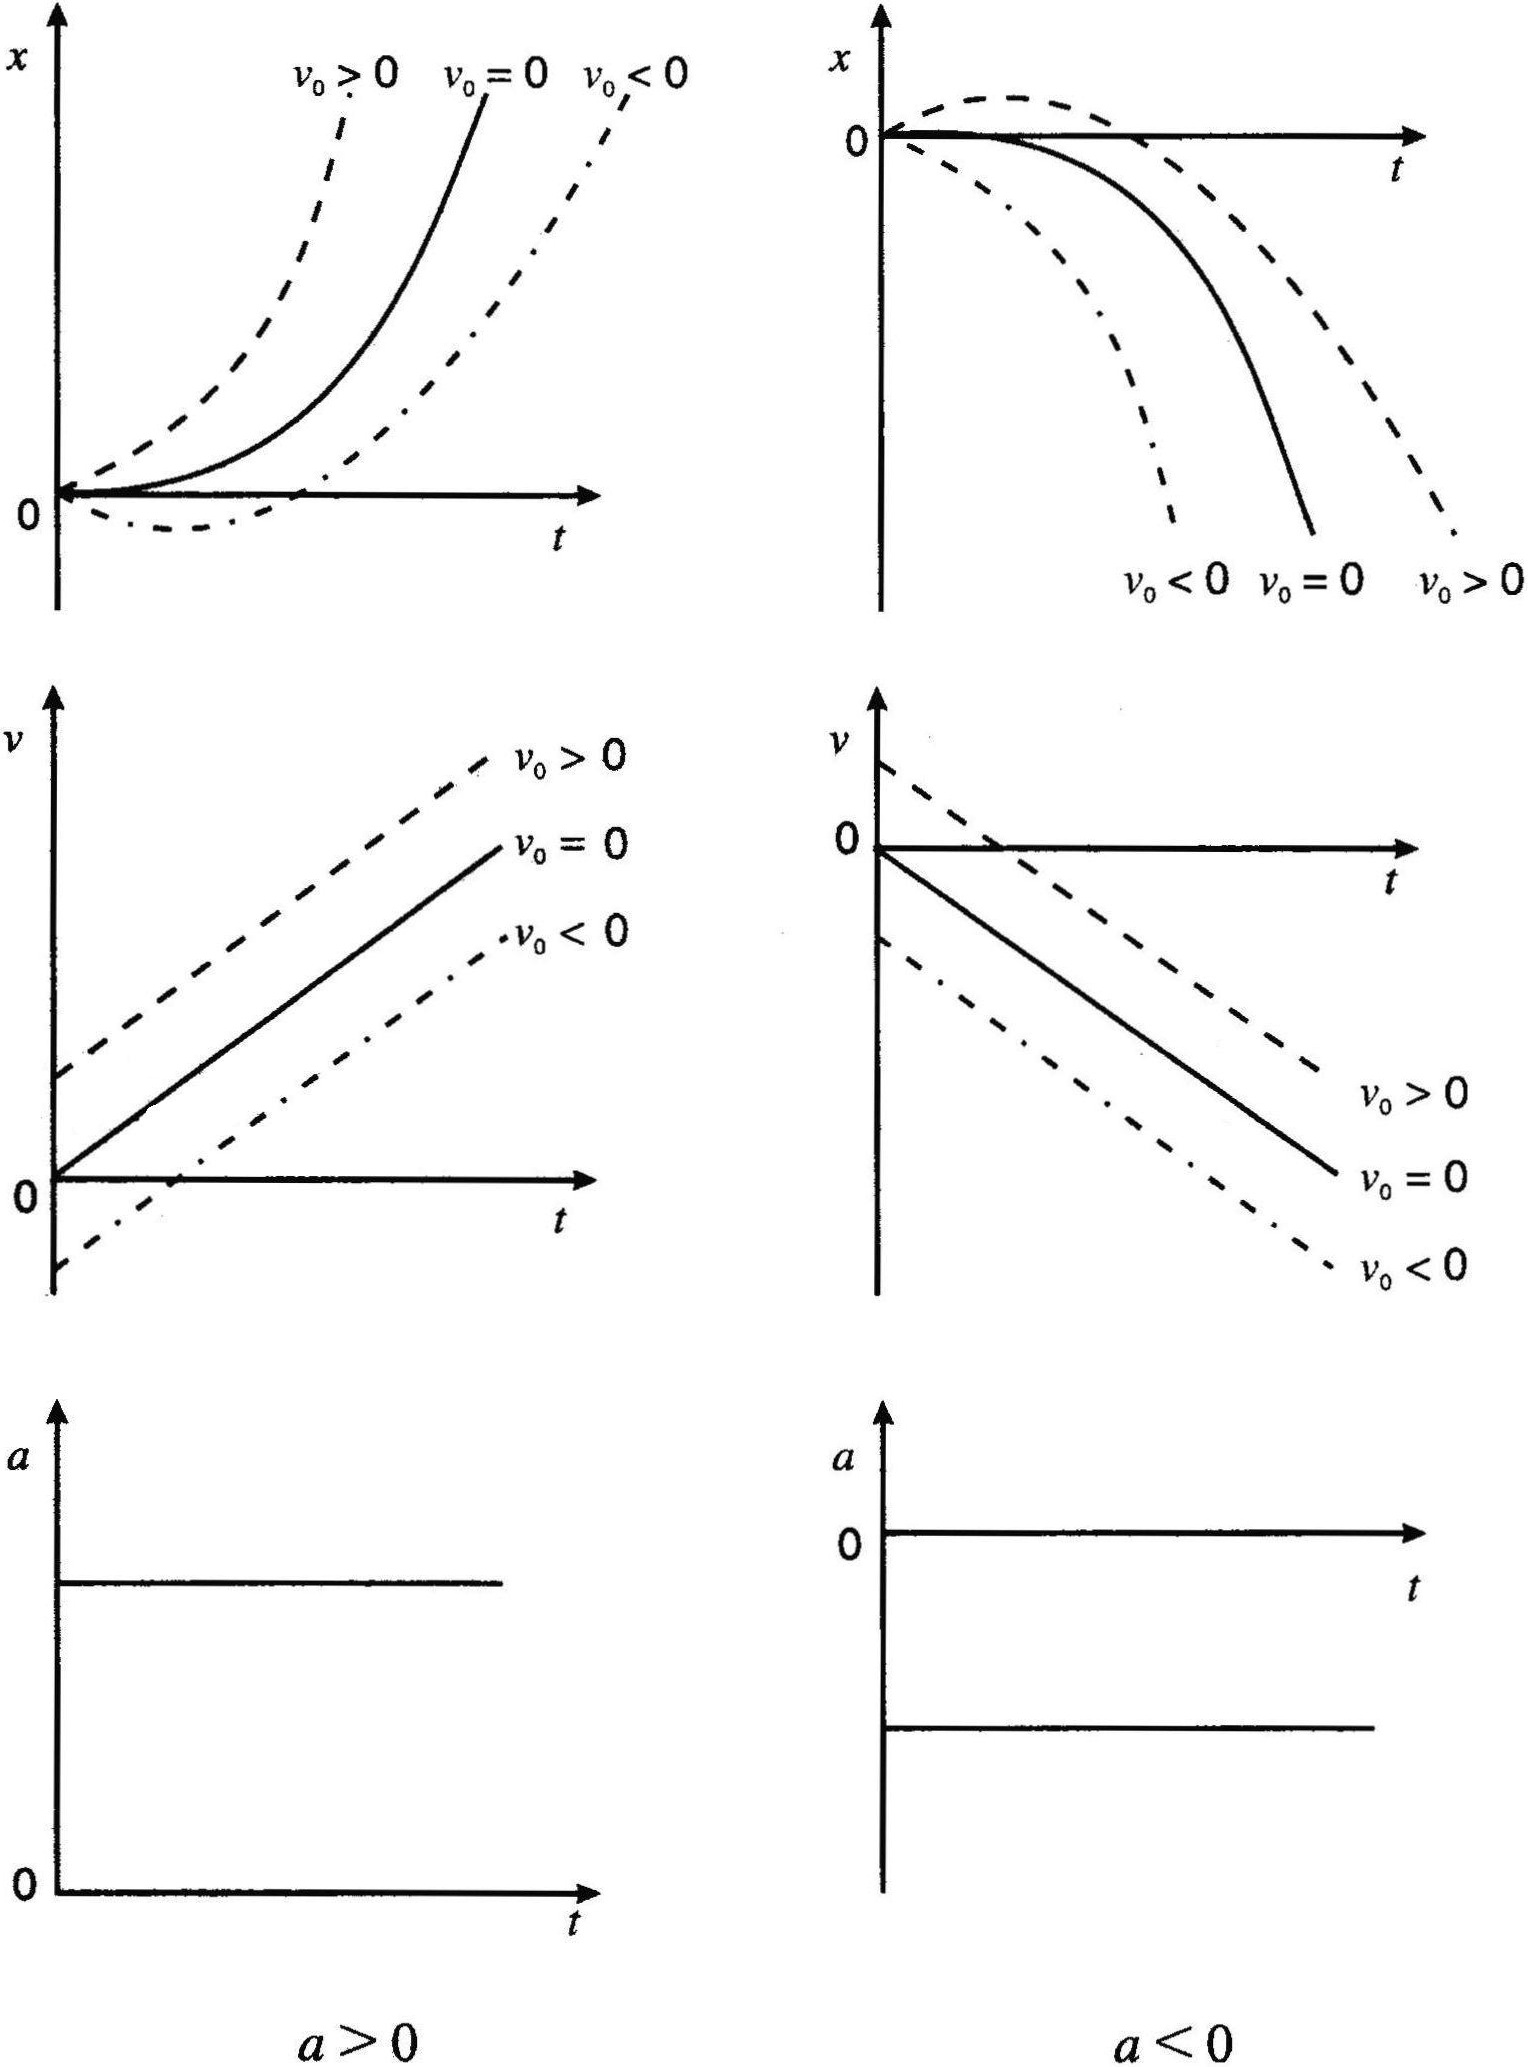
\includegraphics[height=\textheight]{EVRB_grafieken}
\end{image}
\captionof{figure}{Grafieken van een EVRB}




% DEZE CONCEPTUELE VRAAG NOG UITWERKEN 
% \begin{exercise}
% 	\begin{tikzpicture}[scale=5]
% 		% Axes
% 		\draw[->] (-0.05,0) -- (1.1,0) node[right] {$t(s)$};
% 		\draw[->] (0,-0.05) -- (0,1.1) node[above] {$v(s)$};
		
% 		% Grid lines (optional)
% 		\draw[very thin,color=gray!30] (0,0) grid (1,1);
		
% 		% Identity function
% 		\draw[thick,blue,domain=0:1] plot(\x,\x);
% 		\draw[thick,blue,domain=0:1] plot(\x,{pow(\x,2)});
% 		\draw[thick,blue,domain=0:1] plot(\x,{pow(\x,1/2)});
% 		% \draw[thick,red,domain=0:1] plot(\x,{pow(\x,3)});
% 		% \draw[thick,green,domain=0:1] plot(\x,{pow(\x,1/3)});
% 		\draw[thick,blue,domain=0:1] plot(\x,{pow(\x,4)});
% 		\draw[thick,blue,domain=0:1] plot(\x,{pow(\x,1/4)});
		
		
% 	\end{tikzpicture}
% \end{exercise}

\begin{exercise}
	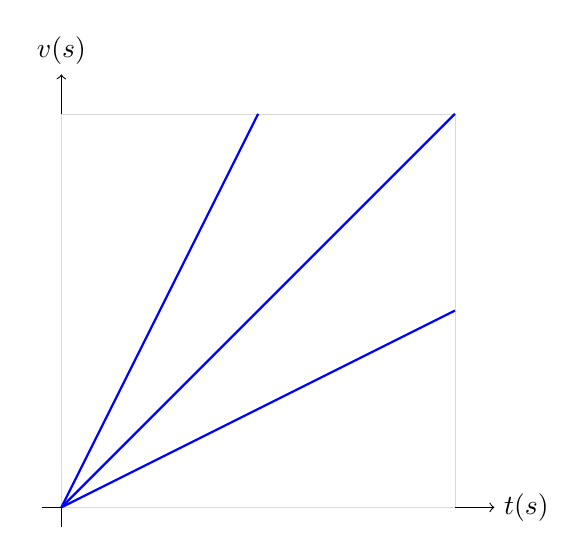
\begin{tikzpicture}[scale=5]
		% Axes
		\draw[->] (-0.05,0) -- (1.1,0) node[right] {$t(s)$};
		\draw[->] (0,-0.05) -- (0,1.1) node[above] {$v(s)$};
		
		% Grid lines (optional)
		\draw[very thin,color=gray!30] (0,0) grid (1,1);
		
		% Identity function
		\draw[thick,blue,domain=0:1] plot(\x,\x);
		\draw[thick,blue,domain=0:(0.5)] plot(\x,{2*\x});
		\draw[thick,blue,domain=0:1] plot(\x,{0.5*\x});
	\end{tikzpicture}
\end{exercise}

\begin{exercise}
	\begin{tikzpicture}[scale=5]
		% Axes
		\draw[->] (-0.05,0) -- (1.1,0) node[right] {$t(s)$};
		\draw[->] (0,-0.05) -- (0,1.1) node[above] {$v(s)$};
		
		% Grid lines (optional)
		\draw[very thin,color=gray!30] (0,0) grid (1,1);
		
		% Identity function
		\draw[thick,blue,domain=0:1] plot(\x,0);
		\draw[thick,blue,domain=0:1] plot(\x, 0.3);
		\draw[thick,blue,domain=0:1] plot(\x,0.8);
	\end{tikzpicture}
\end{exercise}
	

\begin{exercise}

Een auto die $\SI{60}{km/h}$ rijdt, raakt een boom; de voorkant van de auto wordt in elkaar gedrukt en de bestuurder komt na $\SI{70}{cm}$ tot stilstand. Welke gemiddelde vertraging onderging de bestuurder tijdens de botsing? Druk je antwoord uit in $g$, waarbij $g=\SI{9,81}{m/s^2}$.
% \textit{Gegeven}  $v_0=\SI{16,7}{m/s}$%%%\newline$x=\SI{0,70}{m}$
% \textit{Gevraagd} $a$
% \textit{Oplossing} 
\begin{oplossing} 
Om de (constante) vertraging te vinden, hebben we de snelheidsverandering en de benodigde tijd nodig. De verandering in snelheid kennen we; de eindsnelheid van de auto moet nul worden maar de duur is niet onmiddellijk gegeven. Omdat de eindsnelheid nul is, kunnen we wel uit de snelheidsvergelijking van een eenparig veranderlijke beweging een \emph{uitdrukking} vinden voor die tijd die we vervolgens kunnen substitueren in de plaatsvergelijking. De enige onbekende is dan de gezochte versnelling.\footnote{M.b.v. de formule $\overline{v}=\frac{v_0+v}{2}$ voor de gemiddelde snelheid en de definitie voor de gemiddelde snelheid $\overline{v}=\frac{\Delta x}{\Delta t}$ is het antwoord sneller te vinden. Ga maar na \ldots}
%%%\newline
%%%\newline
Uit $v(t)=0$ of $0=v_0+at$ halen we een uitdrukking voor de tijd die nodig is om tot stilstand te komen:
\begin{align*}
t&=-\frac{v_0}{a}
\end{align*}
Substitutie van deze tijd in de plaatsfunctie levert:
\begin{align*}
x&=v_0t+\frac{1}{2}at^2\\
&=v_0\left(-\frac{v_0}{a}\right)+\frac{1}{2}a\left(-\frac{v_0}{a}\right)^2\\
%&=&-\frac{v_0^2}{a}+\frac{v_0^2}{2a}\\
&=-\frac{v_0^2}{2a}\\
\end{align*}
De versnelling is dan gelijk aan:
\begin{align*}
a&=-\frac{v_0^2}{2x}
\end{align*}
Invullen van de gegevens levert $a=\SI{-198}{m/s^2}$, wat gelijk is aan $20g$.
\end{oplossing}
\end{exercise}


	
\end{document}



% Giancoli: 



% We now examine the situation when the magnitude of the acceleration is constant and the motion is in a straight line. In this case, the instantaneous and average accelerations are equal. We use the definitions of average velocity and acceleration to derive a set of valuable equations that relate \( x, v, a, \) and \( t \) when \( a \) is constant, allowing us to determine any one of these variables if we know the others.

% To simplify our notation, let us take the initial time in any discussion to be zero, and we call it \( t_0 \): \( t_1 = t_0 = 0 \). (This is effectively starting a stopwatch at \( t_0 \).) We can then let \( t_2 = t \) be the elapsed time. The initial position (\( x_1 \)) and the initial velocity (\( v_1 \)) of an object will now be represented by \( x_0 \) and \( v_0 \), since they represent \( x \) and \( v \) at \( t = 0 \). At time \( t \), the position and velocity will be called \( x \) and \( v \) (rather than \( x_2 \) and \( v_2 \)).

% The average velocity during the time interval \( t - t_0 \) will be (Eq. 2–2)
% \[
% \bar{v} = \frac{\Delta x}{\Delta t} = \frac{x - x_0}{t - t_0} = \frac{x - x_0}{t}
% \]

% since we chose \( t_0 = 0 \). The acceleration, assumed constant in time, is (Eq. 2–5)

% \[
% a = \frac{v - v_0}{t}
% \]

% A common problem is to determine the velocity of an object after any elapsed time \( t \), when we are given the object's constant acceleration. We can solve such problems by solving for \( v \) in the last equation to obtain:

% \[
% v = v_0 + at \qquad \text{[constant acceleration] (2–7)}
% \]

% If an object starts from rest (\( v_0 = 0 \)) and accelerates at \( 4.0\,\mathrm{m/s^2} \), after an elapsed time \( t = 6.0\,\mathrm{s} \) its velocity will be 
% \[
% v = at = (4.0\,\mathrm{m/s^2})(6.0\,\mathrm{s}) = 24\,\mathrm{m/s}.
% \]

% Next, let us see how to calculate the position \( x \) of an object after a time \( t \) when it undergoes constant acceleration. The definition of average velocity (Eq. 2–2) is
% \[
% \bar{v} = \frac{x - x_0}{t}
% \]
% which we can rewrite as

% \[
% x = x_0 + \bar{v}t \tag{2–8}
% \]

% Because the velocity increases at a uniform rate, the average velocity \( \bar{v} \) will be midway between the initial and final velocities:

% \[
% \bar{v} = \frac{v_0 + v}{2} \qquad \text{[constant acceleration] (2–9)}
% \]

% (Careful: Equation 2–9 is not necessarily valid if the acceleration is not constant.)

% We combine the last two Equations with Eq. 2–7 and find:

% \begin{align*}
% x &= x_0 + \bar{v}t \\
%   &= x_0 + \left( \frac{v_0 + v}{2} \right)t \\
%   &= x_0 + \left( \frac{v_0 + v_0 + at}{2} \right)t \\
%   &= x_0 + v_0 t + \frac{1}{2} at^2
% \end{align*}

% \[
% \Rightarrow \quad x = x_0 + v_0 t + \frac{1}{2}at^2 \qquad \text{[constant acceleration] (2–10)}
% \]
